\section{Multivariate amplitude distributions}
\label{sec:epochs}

In Sect. \ref{subsec:key_concepts} we introduce the fundamental quantities
used in the distribution definitions. An example of the non-stationarity in
financial markets is shown in Sect. \ref{subsec:non_stationarity}. Finally, in
\ref{subsec:epochs} we explain the methodology to see how the returns are to a
good approximation multivariate Gaussian distributed or multivariate Algebraic
distributed.

%%%%%%%%%%%%%%%%%%%%%%%%%%%%%%%%%%%%%%%%%%%%%%%%%%%%%%%%%%%%%%%%%%%%%%%%%%%%%%%
\subsection{Key concepts}\label{subsec:key_concepts}

Consider time series $S_{k} \left( t \right)$, $k = 1, 2, \ldots, K$ of stock
prices for $K$ companies. The values $S_{k} \left( t \right)$ are taken in
fixed time steps $\Delta t$. In general, the data contain an exponential
increase due to the drift. Thus, to measure the correlations independently of
this trend, it is better to use logarithmic differences instead of returns
\begin{equation}
    G_{k} \left( t \right) = \ln S_{k} \left( t + \Delta t \right) -
    \ln S_{k} \left(t \right) = \ln \frac{S_{k} \left( t + \Delta t \right)}
    {S_{k} \left(t \right)}.
\end{equation}
Anyway, logarithmic differences and returns almost coincide if the time steps
$\Delta t$ are sufficiently short \cite{subtle_nature,empirical_facts}
\begin{equation}
    G_{k} \left(t\right) \approx r_{k} \left(t\right)
    = \frac{S_{k} \left( t + \Delta t \right) - S_{k} \left( t \right)}
    {S_{k} \left( t \right)}.
\end{equation}
The returns are well known to have distributions with heavy tails, the smaller
$\Delta t$, the heavier \cite{non_stationarity_fin_guhr}. Furthermore, the
sample standard deviations $\sigma_{k}$, referred to as volatilities, strongly
fluctuate for different time windows of the same length $T$
\cite{non_stationarity_fin_guhr,volatility_change}.

The mean of the logarithmic differences reads \cite{exact_distributions_guhr}
\begin{equation}
    \left\langle G_{k} \left( t \right) \right\rangle_{T} = \frac{1}{T}
    \sum_{t = 1}^{T} G_{k} \left( t \right).
\end{equation}
To compare the different $K$ companies, it is necessary to normalize the time
series. The normalized time series are defined by
\cite{non_stationarity_fin_guhr,exact_distributions_guhr}
\begin{equation}
    M_{k} \left( t \right) = \frac{G_{k} \left( t \right) - \left\langle
    G_{k} \left( t \right) \right\rangle} {\sqrt{\left\langle G_{k}^{2}
    \left( t \right) \right\rangle_{T} - \left\langle G_{k} \left( t \right)
    \right\rangle^2_{T}}},
\end{equation}
where
\begin{equation}
    \sigma_{k} = \sqrt{\left\langle G_{k}^{2}
    \left( t \right) \right\rangle_{T} - \left\langle G_{k} \left( t \right)
    \right\rangle^2_{T}}
\end{equation}
is the volatility of the $k$ company in the time window of length $T$. These
values can be viewed as the elements of a $K \times T$ rectangular matrix $M$.
With these normalizations and rescalings, it can be measured correlations in
such a way that all companies and all stocks are treated on equal footing.

The correlation coefficient for the stocks $k$ and $l$ is defined as
\cite{non_stationarity_fin_guhr}
\begin{equation}
    C_{kl} = \left\langle M_{k} \left( t \right) M_{l} \left( t \right)
    \right\rangle_{T} = \frac{1}{T} \sum_{t=1}^{T} M_{k} \left( t \right) M_{l}
    \left( t \right),
\end{equation}
which can be written as
\begin{equation}
    C_{kl} = \frac{\left\langle G_{k} \left( t \right) G_{l} \left( t \right)
    \right\rangle_{T} - \left\langle G_{k} \left( t \right) \right\rangle_{T}
    \left\langle G_{l} \left( t \right) \right\rangle_{T}}
    {\sigma_{k} \sigma_{l}}.
\end{equation}
The coefficients $C_{kl}$ are the elements of a $K \times K$ square matrix $C$,
the correlation matrix. The limiting values of these correlation coefficients
\begin{equation}
    C_{kl}^{\text{lim}} =
    \left\{
    \begin{array}{cc}
    +1 & \text{completely correlated}  \\
    0  & \text{completely uncorrelated}\\
    -1 & \text{completely anticorrelated}
    \end{array}
    \right. .
\end{equation}
The time average of $C_{kl}$ can be viewed as the matrix product of the
rectangular matrix $M$ ($K \times T$) with its transpose matrix $M^{\dagger}$
($T \times K$), divided by $T$. Thus, the correlation matrix can be written in
the form
\begin{equation}
    C = \frac{1}{T} M M^{\dagger}.
\end{equation}
The correlation matrix $C$ is real and symmetric. Using the correlation matrix
$C$ is possible to define the covariance matrix
\cite{exact_distributions_guhr,credit_risk_guhr,portfolio_distributions_guhr,asset_correlations_guhr,stochastic_cov_guhr}
\begin{equation}
    \Sigma = \sigma C \sigma ,
\end{equation}
where the diagonal matrix $\sigma$ contains respectively, the volatilities
$\sigma_{k}$, $k = 1, \ldots, K$.

\textcolor{red}{I think this is maybe not true. Should we remove this
paragraph?}
From the results obtained in
\cite{non_stationarity_fin_guhr,portfolio_distributions_guhr}, it does not make
a difference the calculation with a covariance or a correlation matrix. Thus,
to ease the comparison between works, we will use covariance matrices as in
\cite{non_stationarity_fin_guhr}.

%%%%%%%%%%%%%%%%%%%%%%%%%%%%%%%%%%%%%%%%%%%%%%%%%%%%%%%%%%%%%%%%%%%%%%%%%%%%%%%
\subsection{Non-stationarity}\label{subsec:non_stationarity}

In general, in non-stationary complex systems crucial parameters or
distributions of observables change in an erratic, unpredictable way over time.
In financial markets, the change of the $K \times K$ correlation matrix $C$ as
a whole in time is an example of non-stationary. Fig.
\ref{fig:correlation_matrices} shows two large correlation matrices of
logarithmic differences of stock prices for companies in the Standard \&
Poor's 500 (S\&P 500) stock market index ordered according to the Global
Industry Classification Standard (GICS). The time series were measured in
successive quarters. The stripes in these correlation matrices indicate the
structuring of the market in industrial sectors
\cite{state_crisis_7,non_stationarity_fin_guhr}

\begin{figure}[htbp]
    \centering
    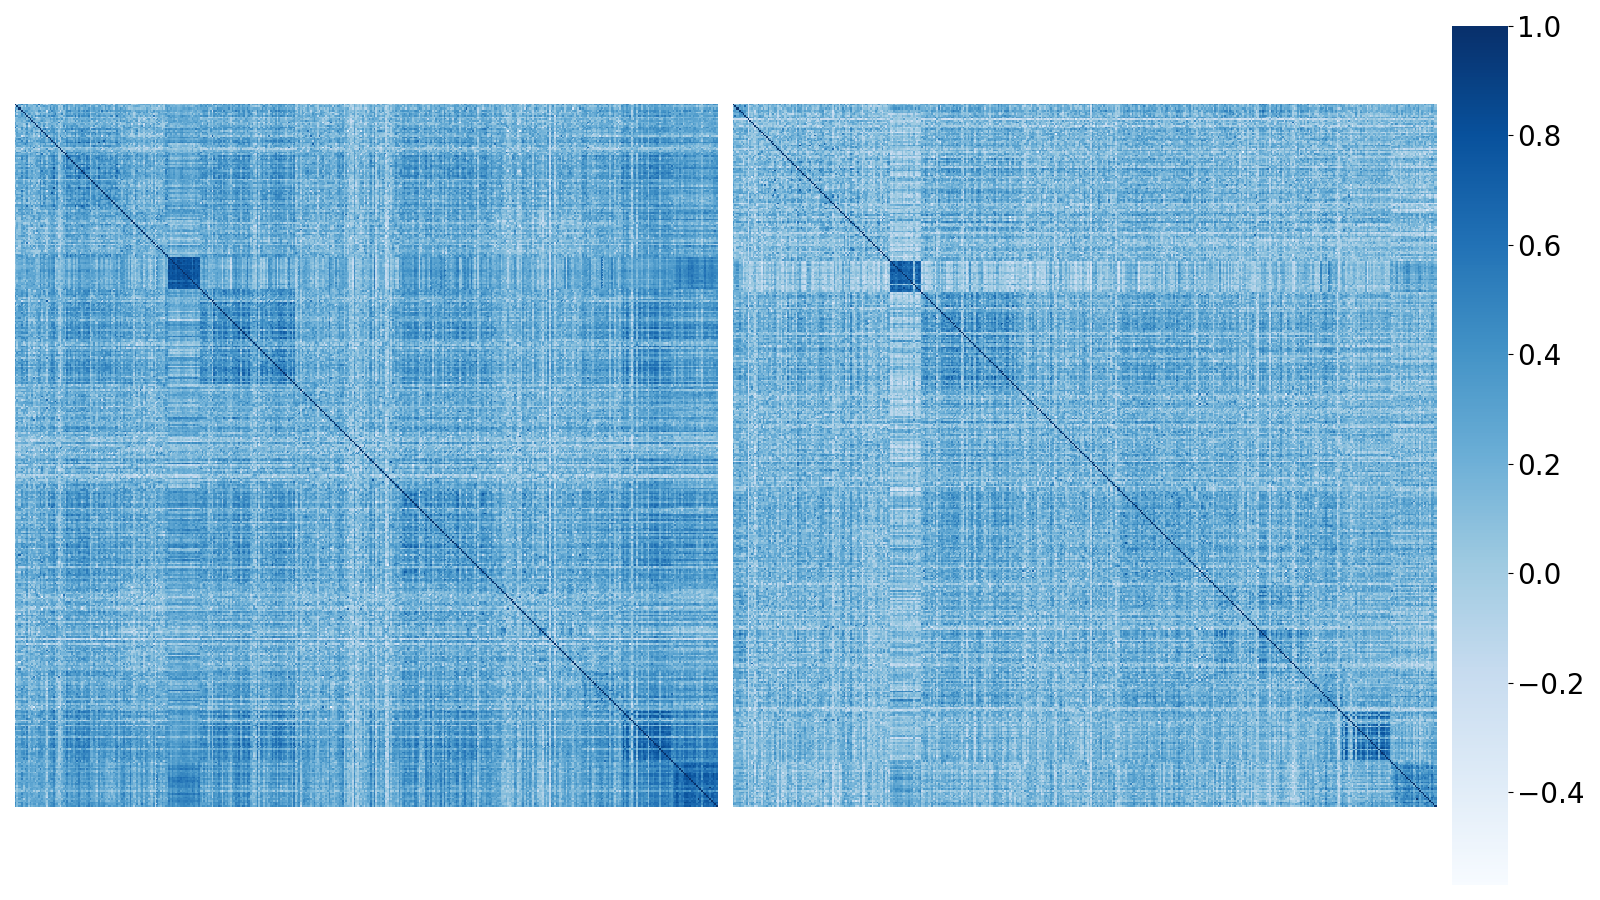
\includegraphics[width=0.6\columnwidth]
    {figures/05_correlation_matrix.png}
    \caption{Correlation matrices of $K = 421$ companies for the fourth quarter
             of 2005 (left) and the first quarter of 2006 (right), the darker,
             the stronger the correlation. The companies are sorted according
             to industrial sectors.}
    \label{fig:correlation_matrices}
\end{figure}

In Fig. \ref{fig:correlation_matrices} it can be seen that the matrices look
different for the successive quarters, because the business relations between
the companies and the market expectations of the traders change in time.
Despite the difference, the coarse structure remains similar, indicating some
stability of the industrial sectors.

%%%%%%%%%%%%%%%%%%%%%%%%%%%%%%%%%%%%%%%%%%%%%%%%%%%%%%%%%%%%%%%%%%%%%%%%%%%%%%%
\subsection{Choice of amplitude in each of the epochs}\label{subsec:epochs}

We use the same methodology from T. A. Schmitt et al.
\cite{non_stationarity_fin_guhr} to show that to a good approximation, the
returns can be multivariate Gaussian distributed or multivariate algebraic
distributed, depending of the epochs window length choice. All of this, if the
covariance matrix $\Sigma$ is fixed within the epochs.

We start from the assumption that the $K$ dimensional vectors
$r \left( t \right) = \left( r_{1} \left( t \right), \ldots, r_{K} \left( t \right) \right)$
for a fixed return interval $\Delta t$ is given by the multivariate Gaussian
distribution
\begin{equation}\label{eq:gaussian_distribution}
    P_{G} \left( r| \Sigma_{ep} \right) =
    \frac{1}{\sqrt{\det 2 \pi \Sigma_{ep} }}
    \exp \left( - \frac{1}{2} r^{\dagger} \Sigma_{ep}^{-1} r \right).
\end{equation}
To test the assumption, we divide the time series in windows of length $T$
where the sampled covariances can be viewed as constant within these windows.

To carry out the data analysis, whether for the multivariate Gaussian
distribution or the multivariate Algebraic distribution, we choose all pairs of
returns, normalize the epochs (mean $\mu = 0$ and variance $\sigma^{2} = 1$)
and create two-component vectors
$\left( r_{k} \left( t \right), r_{l} \left( t \right) \right)$. For each pair,
we evaluate the $2 \times 2$ sample covariance matrix
$\Sigma^{\left(k, l \right)}$. Then we diagonalize the covariance matrix as
$\Sigma = U \Lambda U^{\dagger}$, such that
$\Sigma^{-1/2} = U \Lambda^{-1/2} U^{\dagger}$, where $U$ is an orthogonal
$K \times K$  matrix and $\Lambda$ is the diagonal matrix of the eigenvalues
$\Lambda_{K}$. We rotate the two-component returns vectors into the eigenbasis
of $\Sigma^{\left(k, l \right)}$,
\begin{equation}
    \left(\tilde{r}_{1} \left(t \right), \tilde{r}_{2} \left(t \right) \right)
    = U \left(r_{k} \left(t \right), r_{l} \left(t \right) \right)
\end{equation}
and normalize the axis with the eigenvalues as
\begin{equation}
    \frac{\tilde{r}_{1} \left(t \right)}{\sqrt{\Lambda_{1}}} \text{ and }
    \frac{\tilde{r}_{2} \left(t \right)}{\sqrt{\Lambda_{2}}}.
\end{equation}
Finally, we aggregate all the components into a single univariate distribution,
as all of them are now comparable.

Now we need to find the one dimensional function related to the multivariate
Gaussian distribution in Eq. \ref{eq:gaussian_distribution} to compare with the
empirical  single univariate distributions. In the Gaussian case, we know that
\begin{align}
    P_{G}^{\left( ij \right)} \left( r^{\left( ij \right)} |
    \Sigma_{ep}^{\left( ij \right)} \right)
    &= \int d \left[ r \right]_{\ne i,j} P_{G} \left( r | \Sigma_{ep} \right)\\
    &= \frac{1}{\sqrt{\det 2 \pi \Sigma_{ep}^{\left( ij \right)}}}
    \exp \left( -\frac{1}{2} r^{\left( ij \right) \dagger}
    \Sigma_{ep}^{\left( ij \right)^{ - 1}} r^{\left( ij \right)} \right)
\end{align}
is the corresponding bivariate model where
\begin{equation}
    r^{\left(ij\right)}=\left[\begin{array}{c}
    r_{i}\\
    r_{j}
    \end{array}\right]\text{ and } \Sigma_{ep}^{\left(ij\right)}
    =\left[\begin{array}{cc}
    \Sigma_{ep,ii} & \Sigma_{ep,ij}\\
    \Sigma_{ep,ji} & \Sigma_{ep,jj}
    \end{array}\right]
\end{equation}
are the two-component return vector and the $2 \times 2$ covariance matrix.
$\Sigma_{ep,ij}$ is just the $\left( ij \right)$ element of $\Sigma_{ep}$.
Diagonalising
\begin{equation}
    \Sigma_{ep}^{\left(ij\right)}=U^{\left(ij\right)}
    \Lambda_{ep}^{\left(ij\right)}U^{\left(ij\right)\dagger}
\end{equation}
with the $2 \times 2$ rotation matrix $U^{\left( ij \right)}$ and the
eigenvalue matrix
\begin{equation}
    \Lambda_{ep}^{\left( ij \right)} = \text{diag}
    \left( \Lambda_{ep,1}^{\left( ij \right)},
    \Lambda_{ep,2}^{\left( ij \right)} \right).
\end{equation}
We rotate into the eigenbasis
\begin{equation}
    \bar{r}^{\left(ij\right)}=\left[\begin{array}{c}
    \bar{r}_{1}^{\left(ij\right)}\\
    \bar{r}_{2}^{\left(ij\right)}
    \end{array}\right]=U^{\left(ij\right)\dagger}r^{\left(ij\right)}
\end{equation}
such that
\begin{align}
    P_{G}^{\left(ij\right)}\left(r^{\left(ij\right)}|
    \Sigma_{ep}^{\left(ij\right)}\right)
    &=P_{G}^{\left(ij\right)}\left(\bar{r}^{\left(ij\right)}|
    \Lambda_{ep}^{\left(ij\right)}\right)\\
    &=\frac{1}{\sqrt{2\pi\Lambda_{ep,1}^{\left(ij\right)}}}
    \exp\left(-\frac{\bar{r}_{1}^{\left(ij\right)^{2}}}{2\Lambda_{ep,1}
    ^{\left(ij\right)}}\right)
    \,\frac{1}{\sqrt{2\pi\Lambda_{ep,2}^{\left(ij\right)}}}
    \exp\left(-\frac{\bar{r}_{2}^{\left(ij\right)^{2}}}{2\Lambda_{ep,2}
    ^{\left(ij\right)}}\right).
\end{align}
The univariate rotated distribution is
\begin{align}
    \tilde{P}_{G}^{\left(ij\right)}\left(\tilde{r}\right)
    &=\intop_{-\infty}^{+\infty}d\bar{r}_{2}^{\left(ij\right)}
    P_{G}^{\left(ij\right)}\left(\bar{r}^{\left(ij\right)}|
    \Lambda_{ep}^{\left(ij\right)}\right)\vert_{\bar{r}_{1}^{\left(ij\right)}/
    \sqrt{\Lambda_{ep,1}^{\left(ij\right)}}=\tilde{r}}\,
    \frac{d\bar{r}_{1}^{\left(ij\right)}}{d\tilde{r}}\\
    & =\frac{1}{\sqrt{2\pi}}\exp\left(-\frac{1}{2}\tilde{r}^{2}\right),
\end{align}
which is the standard Gaussian distribution with mean $\mu = 0$ and variance
$\sigma^2 = 1$.

To check the validity of our assumption, in Fig.
\ref{fig:gaussian_agg_returns_epoch} we plot the daily adjusted closing
aggregated returns distribution of 200 companies from the S\&P 500 dataset,
with a $\Delta t = 1d$ and an epoch window length $T = 25d$. For the
univariate distribution case we observe a good agreement with the one
dimensional Gaussian distribution, as expected.

\begin{figure}[htbp]
    \centering
    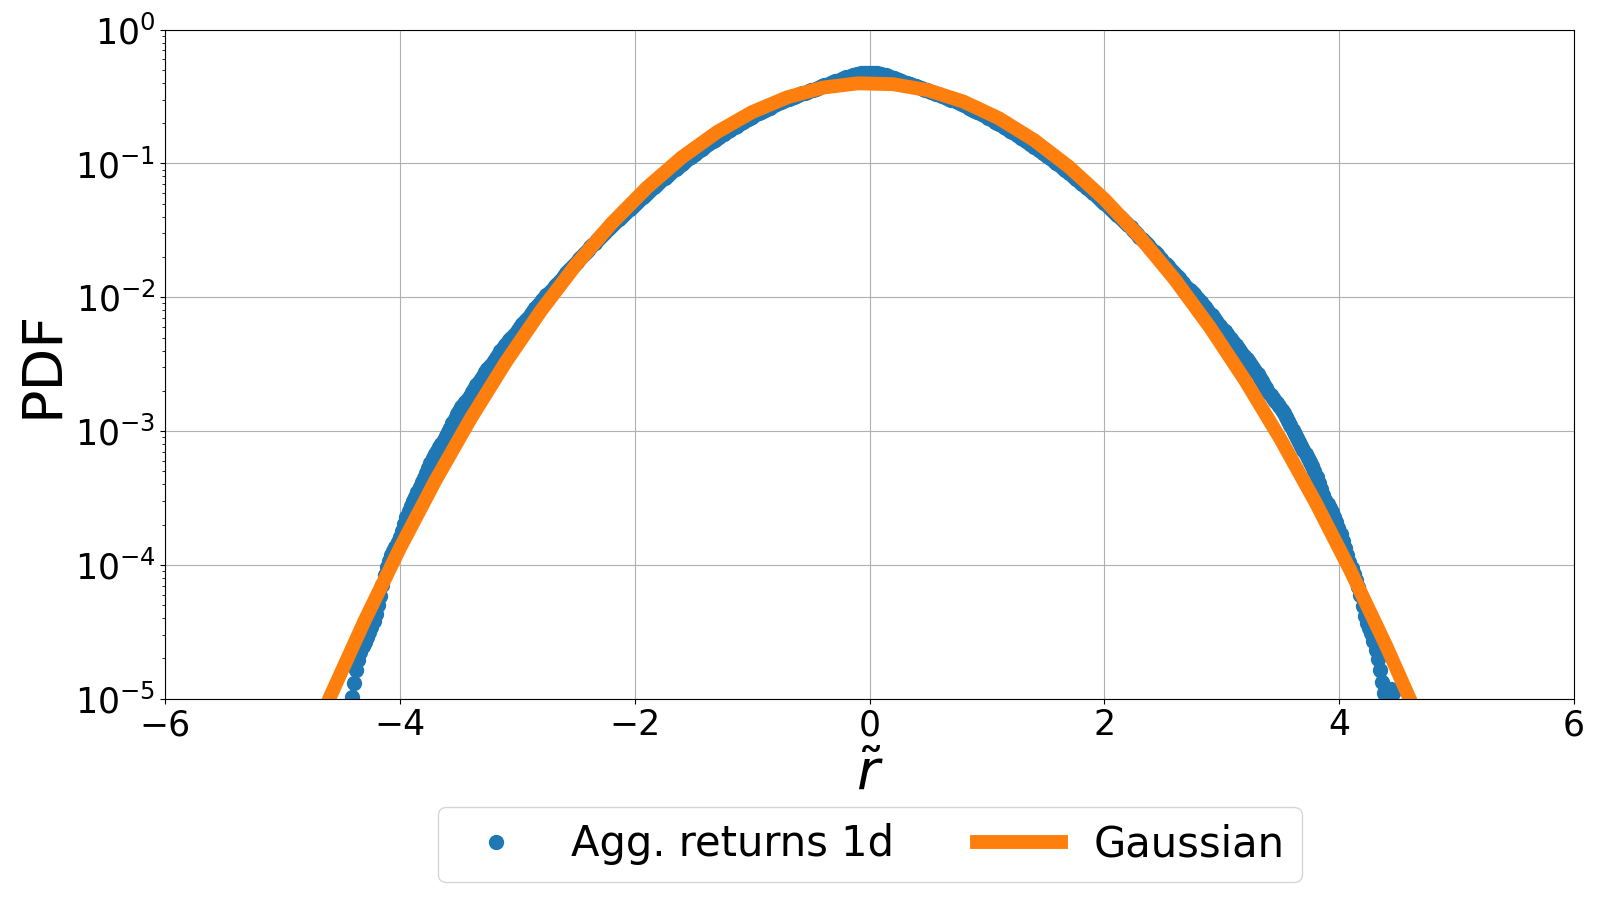
\includegraphics[width=0.6\columnwidth]
    {figures/05_gaussian_agg_returns_short_epoch.png}
    \caption{[CAMBIAR IMAGEN] Aggregated distribution of returns ($\tilde{r}$) for fixed
             covariance of 200 companies selected from the S\&P 500
             dataset. $\Delta t = 1d$ and epoch window length $T=25d$.}
    \label{fig:gaussian_agg_returns_epoch}
\end{figure}

To model heavy tails, we assume that the $K$ dimensional vectors
$r \left( t \right) = \left( r_{1} \left( t \right), \ldots, r_{K} \left( t \right) \right)$
for a fixed return interval $\Delta t$ is given by the multivariate algebraic
distribution
\begin{align}
    P_{A} \left( r | \Sigma_{ep} \right)
    &= \frac{\alpha_{K1lm}}{\left( 1 + \frac{1}{m} r^{\dagger}
    \Sigma^{-1}_{ep} r \right)^{l}}\label{eq:algebraic_distribution} \\
    \alpha_{K1lm} &= {\sqrt{\frac{2}{m}}}^{K}
    \frac{\Gamma \left( l \right)}{\Gamma \left( l - K/2 \right)}
    \frac{1}{\sqrt{\det 2 \pi \Sigma_{ep}}}.
\end{align}
To test the new assumption and compare the different time step data, we repeat
the same method to rotate and scale the returns to then get the aggregate
distribution of returns. Once more, we need to find the corresponding one
dimensional functions related to the multivariate algebraic distribution in Eq.
\ref{eq:algebraic_distribution} to compare with the empirical single univariate
distributions.

We know that the algebraic model from Eq. \ref{eq:algebraic_distribution}
relates to the Gaussian model from Eq. \ref{eq:gaussian_distribution} via
\begin{equation}
    P_{A}\left(r|\Sigma_{ep}\right)
    =\intop_{0}^{\infty}\chi_{2\left(l-K/2\right)}^{2}\left(z\right)\,
    P_{G}\left(r|\frac{m}{2}\Sigma_{ep}\right)dz.
\end{equation}
We immediately find
\begin{align}
    P_{A}^{\left(ij\right)}\left(r^{\left(ij\right)}|
    \Sigma_{ep}^{\left(ij\right)}\right)
    & =\int d\left[r\right]_{\ne i,j}P_{A}\left(r|\Sigma_{ep}\right)\\
    & =\intop_{0}^{\infty}dz\,\chi_{2\left(l-K/2\right)}^{^{2}}\left(z\right)
    \frac{1}{\sqrt{\det2\pi\frac{m}{2}\Sigma_{ep}^{\left(ij\right)}}}
    \exp\left(-\frac{z}{2m}r^{\left(ij\right)\dagger}
    \Sigma_{ep}^{\left(ij\right)^{-1}}r^{\left(ij\right)}\right)\\
    & =\frac{1}{\sqrt{\det2\pi\Sigma_{ep}^{\left(ij\right)}}}
    \intop_{0}^{\infty}dz\,\chi_{2\left(l-K/2\right)}^{^{2}}\left(z\right)
    \frac{z}{m}\exp\left(-\frac{z}{2m}r^{\left(ij\right)\dagger}
    \Sigma_{ep}^{\left(ij\right)^{-1}}r^{\left(ij\right)}\right).
\end{align}
Using
\begin{equation}
    \chi_{q+2}^{2}\left(z\right)=\frac{1}{q}\chi_{q}^{2}\left(z\right)z
\end{equation}
we have
\begin{align}
    P_{A}^{\left(ij\right)}\left(r^{\left(ij\right)}|
    \Sigma_{ep}^{\left(ij\right)}\right)
    &=\frac{2\left(l-K/2\right)}{m\sqrt{\det2\pi\Sigma_{ep}^{\left(ij\right)}}}
    \intop_{0}^{\infty}dz\,\chi_{2\left(l+1-K/2\right)}^{2}\left(z\right)
    \exp\left(-\frac{z}{2m}r^{\left(ij\right)\dagger}
    \Sigma_{ep}^{\left(ij\right)^{-1}}r^{\left(ij\right)}\right)\\
    & =\frac{2\left(l-K/2\right)}{m\sqrt{\det2\pi\Sigma_{ep}
    ^{\left(ij\right)}}}\frac{1}{2^{l+1-K/2}\Gamma\left(l+1-K/2\right)}
    \intop_{0}^{\infty}dz\,z^{l-K/2}
    \exp\left[-\frac{z}{2}\left(1+\frac{1}{m}r^{\left(ij\right)\dagger}
    \Sigma_{ep}^{\left(ij\right)^{-1}}r^{\left(ij\right)}\right)\right]\\
    &=\frac{2l-K}{m\sqrt{\det2\pi\Sigma_{ep}^{\left(ij\right)}}}
    \frac{1}{\left(1+\frac{1}{m}r^{\left(ij\right)\dagger}
    \Sigma_{ep}^{\left(ij\right)^{-1}}r^{\left(ij\right)}\right)^{l+1-K/2}}
    \label{eq:using_chi}.
\end{align}
Rotating into the eigenbasis, we can integrate out one of the variables
\begin{equation}
    \tilde{P}_{A}^{\left(ij\right)}\left(\bar{r}_{1}^{\left(ij\right)}|
    \Lambda_{ep,1}^{\left(ij\right)}\right)
    =\intop_{-\infty}^{+\infty}d\bar{r}_{2}^{\left(ij\right)}
    P_{A}^{\left(ij\right)}\left(\bar{r}^{\left(ij\right)}|
    \Lambda_{ep}^{\left(ij\right)}\right).
\end{equation}
Using Eq. \ref{eq:using_chi}, we have
\begin{align}
    \tilde{P}_{A}^{\left(ij\right)}\left(\bar{r}_{1}^{\left(ij\right)}|
    \Lambda_{ep,1}^{\left(ij\right)}\right)
    &=\frac{2\left(l-K/2\right)}{\sqrt{m}\sqrt{2\pi\Lambda_{ep,1}
    ^{\left(ij\right)}}}\frac{1}{2^{l+1-K/2}\Gamma\left(l+1-K/2\right)}
    \intop_{0}^{\infty}dz\,z^{l-K/2-1/2}\exp\left[-\frac{z}{2}
    \left(1+\frac{1}{m}\frac{\bar{r}_{1}^{\left(ij\right)^{2}}}
    {\Lambda_{ep,1}^{\left(ij\right)}}\right)\right]\\
    &=\frac{2\left(l-K/2\right)}{\sqrt{m}\sqrt{2\pi\Lambda_{ep,1}^
    {\left(ij\right)}}}\frac{2^{l+1/2-K/2}
    \Gamma\left(l+1/2-K/2\right)}{2^{l+1-K/2}
    \Gamma\left(l+1-K/2\right)}\frac{1}{\left(1+\frac{1}{m}
    \frac{\bar{r}_{1}^{\left(ij\right)^{2}}}
    {\Lambda_{ep,1}^{\left(ij\right)}}\right)^{l-\left(K-1\right)/2}}\\
    &=\sqrt{\frac{2}{m}}\frac{\Gamma\left(l-\left(K-1\right)/2\right)}
    {\Gamma\left(l-K/2\right)}\frac{1}{\sqrt{2\pi\Lambda_{ep,1}
    ^{\left(ij\right)}}}\frac{1}{\left(1+\frac{1}{m}
    \frac{\bar{r}_{1}^{\left(ij\right)^{2}}}
    {\Lambda_{ep,1}^{\left(ij\right)}}\right)^{l-\left(K-1\right)/2}}.
\end{align}
Going over to the rescaled variable
\begin{equation}
    \tilde{r} = \frac{\bar{r}^{\left( ij \right)}}{\sqrt{\Lambda_{ep,1}
    ^{\left( ij \right)}}}
\end{equation}
we arrive at
\begin{equation}
    \tilde{P}_{A}^{\left(ij\right)}\left(\tilde{r}\right)
    =\frac{1}{\sqrt{2\pi}}\sqrt{\frac{2}{m}}
    \frac{\Gamma\left(l-\left(K-1\right)/2\right)}{\Gamma\left(l-K/2\right)}
    \frac{1}{\left(1+\frac{1}{m}\tilde{r}^{2}\right)^{l-\left(K-1\right)/2}}
\end{equation}
which is the algebraic distribution to be fitted to the aggregated returns.
In this case we have three parameters: $K$, $l$ and $m$. $K$ is the number of
companies used and is known from the data. $l$ and $m$ are the shape parameters
of the distribution and have to be determined by fitting. In the model, the
expectation value $\langle r r^{\dagger} \rangle$ serves as an estimator for
the sample covariances. We find
\begin{equation}
    \langle r r^{\dagger} \rangle_{Y} = \beta_{Y} \Sigma_{ep}
\end{equation}
with
\begin{equation}
    \beta_{Y}=\begin{cases}
    1, & \text{if }Y=G\\
    \frac{m}{2l-K-2}, & \text{if }Y=A
\end{cases}.
\end{equation}
Due to its very definition, we have $\beta_{G} = 1$ for the multivariate
Gaussian, but a different value $\beta_{A}$ for the algebraic distribution. The
relation in the latter case then suggest the useful fixing
\begin{equation}\label{eq:m_relation}
    m = 2l - K - 2
\end{equation}
also for finite values of $l$ and $m$. Only with this choice, $\Sigma_{ep}$ can
be estimated by the sample covariance matrix, otherwise only up to some factor.

\begin{figure}[htbp]
    \centering
    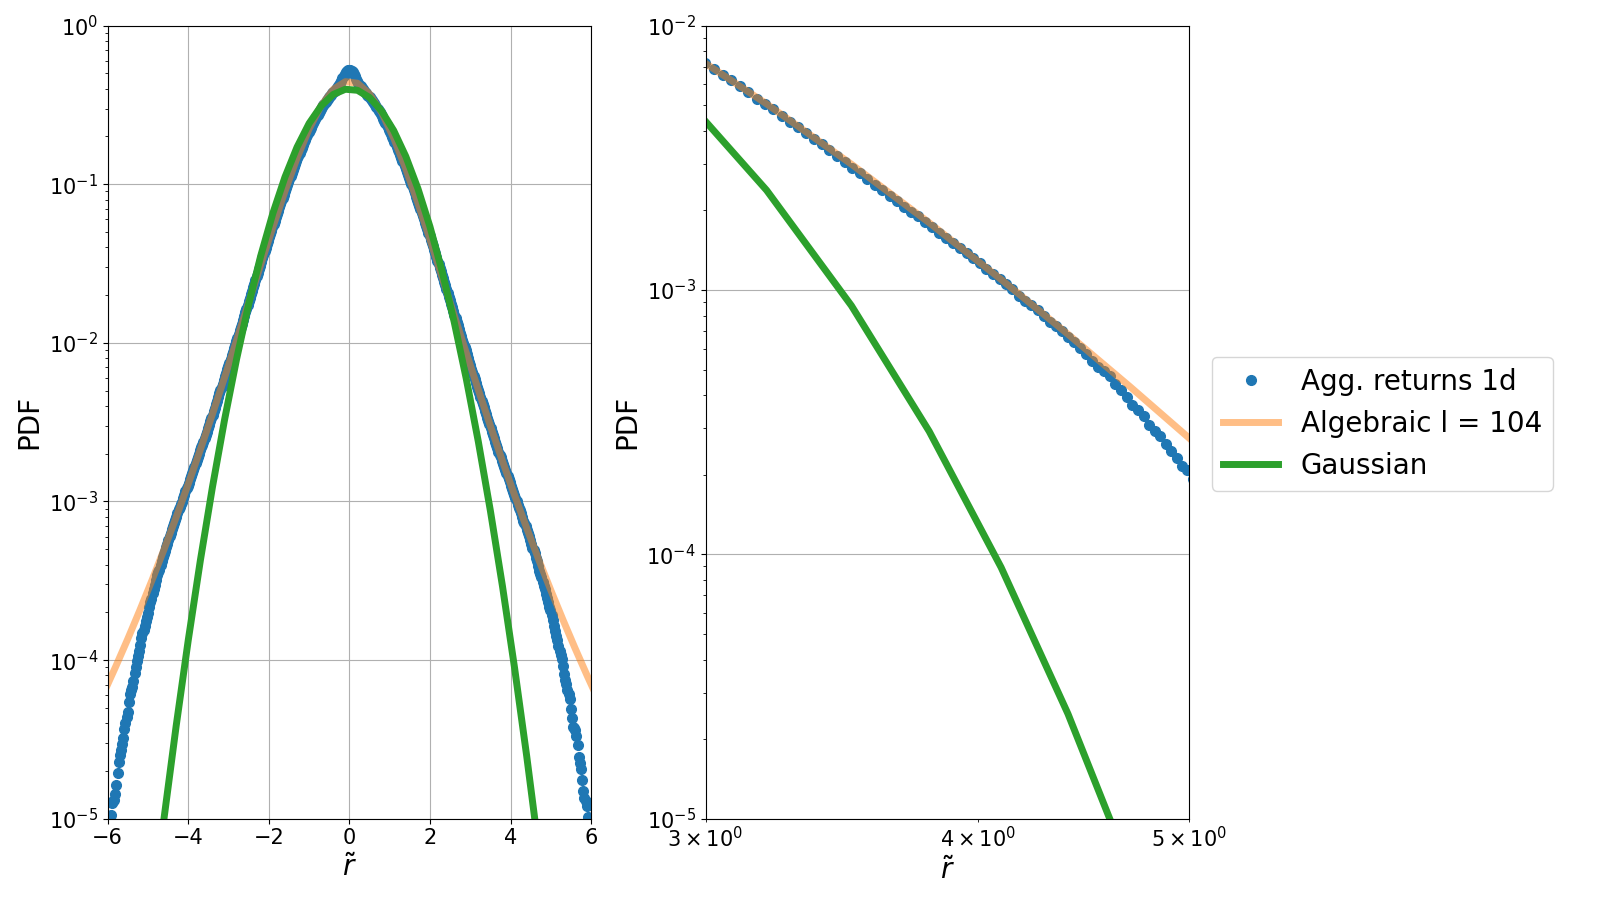
\includegraphics[width=0.7\columnwidth]
    {figures/05_algebraic_agg_returns_short_epoch.png}
    \caption{[CAMBIAR IMAGEN] Semilog plot (left) and loglog plot (right) of the aggregated
             distribution of returns ($\tilde{r}$) for fixed covariance of 200
             companies selected from the S\&P 500 dataset. $\Delta t = 1d$ and
             epoch window length $T=55d$. The empirical data is compared with
             the best fit of one dimensional algebraic distribution with shape
             parameter $l=XX$.}
    \label{fig:algebraic_agg_returns_epoch}
\end{figure}

Having these details in mind and to check the validity of our assumption, in
Fig. \ref{fig:algebraic_agg_returns_epoch} we plot the daily adjusted closing
aggregated returns distribution of 200 companies from the S\&P 500 dataset,
with a $\Delta t = 1d$ and an epoch window length $T = 55d$. Using Eq.
\ref{eq:m_relation} to compute $m$, we found that for one day, $l = 29$ fits
well with the aggregated returns. We plot the one dimensional Gaussian
distribution as a reference.

We know that the aggregated returns have internal Gaussian and algebraic
structures depending on the epochs window length. The larger the value of $T$,
the heavier the tails and the smaller the stationary assumption within the
epochs. However, during the epochs analysis we found an unusual behavior when
we used small epochs window lengths.

Using the methodology described in the work of Schmitt et al.
\cite{non_stationarity_fin_guhr}, we wanted to find which was the best value of
the epochs window length to fit the Gaussian case and the algebraic case. We
use epochs window lengths $T = 10, 25, 40, 55$ days and $\Delta t = 1d$. In
Fig. \ref{fig:window_comparison} can be seen the difference between epochs
window lengths of the aggregated distribution of returns for fixed covariance
of different amount of random companies selected from the S\&P 500 dataset. We
choose random numbers of companies within our dataset to show the independence
of shape related with the number of companies. We can see how for $T=25d$
(top left) there is a good agreement with the Gaussian distribution, and how
for values larger than $T=25d$, as $T=40d$ (bottom left) and $T=55d$
(bottom right), the aggregated returns have fat tails. It is also interesting
how for $T=10d$ (top left), the aggregated returns have a platykurtic behavior.
The results for the aggregated distributions show that their shapes are
independent of the number of companies used and only depend on the length of
the time window length of the epochs. These results are weird, as depending on
the number of companies used, the curves should have different shapes.

\begin{figure}[htbp]
    \centering
    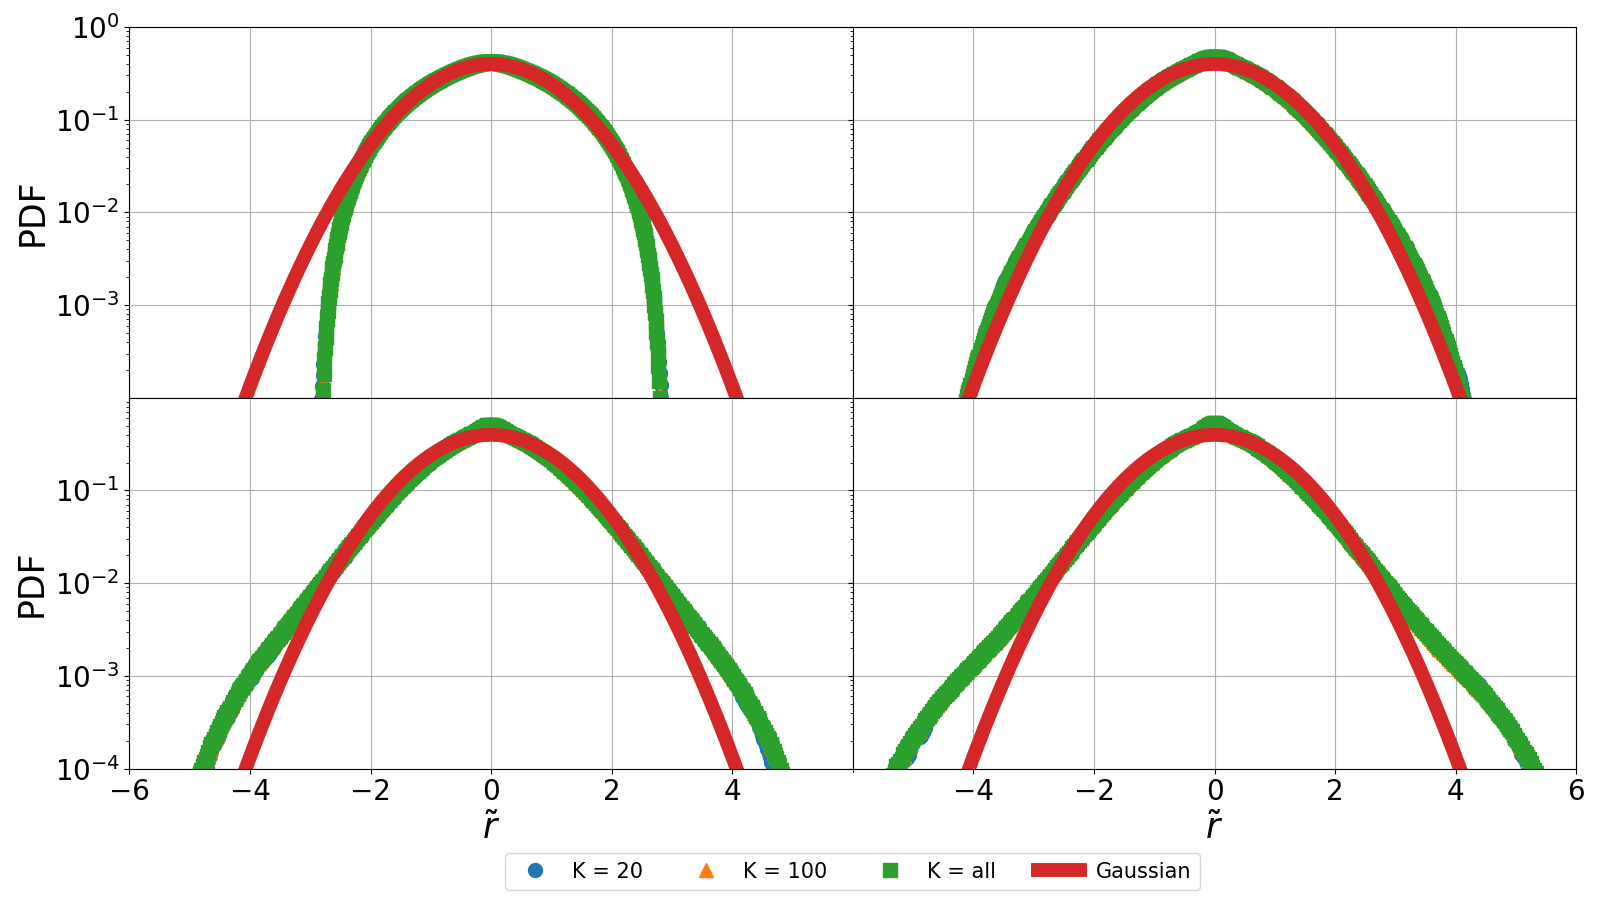
\includegraphics[width=0.8\columnwidth]
    {figures/05_window_comparison.png}
    \caption{[CAMBIAR IMAGEN] Aggregated distribution of returns ($\tilde{r}$) for fixed
             covariance of different number of companies selected from the S\&P
             500 dataset. $\Delta t = 1d$ and different epochs window lengths
             $T=10d$ (top left), $T=25d$ (top right), $T=40d$ (bottom left) and
             $T=55d$ (bottom right).}
    \label{fig:window_comparison}
\end{figure}

We consider three different causes for this situation. First, it could be an
ergodicity defect because only the length of the time window of the epochs show
an effect. Second, the platykurtic behavior like in local normalization plots
\cite{local_normalization} could be a detrending method. It is possible that we
get this behavior from normalizing each epoch to mean
$\mu = 0$ and $\sigma^{2}=1$. Finally, it could be that the rotation and
scaling method has an effect because there should be heavy tails in aggregated
returns without rotation and scaling.

\textcolor{red}{Toni: maybe could you explain here your "guess" from the pdf
document where you say there is a method artifact?}

To check what is the real cause of this behavior we will use simulations.
With these simulations we know which parameters we are using, and we have a
controlled environment. Thus, we can evaluate where is the problem with the
method.